\section{What survives without ground truth}
\label{sec:audit}

We now measure what each layer of the published protocol (\cref{sec:intro}) adds\claim{C-P1}.
The supplement lists the selection protocols of recent work.

\paragraph{FFHQ: nearly everything survives.}
\Cref{tab:ffhq} decomposes the FFHQ results at the run counts of the original experiments.
Residual selection followed by the orientation test recovers $92.6$--$97.5\%$ of the mean-PSNR gain from the first run to the orbit oracle.
It stays within two images of the orbit oracle in the number of \good picks\claim{C-A3}.
At these run counts, the residual pick fails on $84$ of the $540$ image--solver pairs.
The orientation test fixes $14$ of them and breaks none.
Of the remaining $70$, $66$ are images with no \good run in any orientation, $3$ are selection misses, and $1$ is the only partial orbit error among the $1{,}960$ runs\claim{C-A4}.
What does not survive is therefore coverage, not selection.
Coverage depends on the solver.
$57\%$ of SITCOM's failed runs are \cons, against $10\%$ for DAPS-2K and $8\%$ for FAST-DIPS\claim{C-A5}.
This is why stopping helps DAPS and not SITCOM (\cref{sec:protocol}).
Under Gaussian noise, a run's likelihood depends on the measurement only through its residual, so telling a \cons run from a \good one needs the prior, not another residual.

\begin{table}[t]
\centering\footnotesize
\setlength{\tabcolsep}{2.0pt}
\begin{tabular}{@{}lcccccccc@{}}
\toprule
 & & \multicolumn{4}{c}{Mean PSNR (dB)} & & \multicolumn{2}{c}{\good} \\
\cmidrule(lr){3-6}\cmidrule(l){8-9}
Solver (cohort) & $K$ & First & $\Eone$ & $\Oraw$ & $\Oorb$ & Rec. & $\Eone$ & $\Oorb$ \\
\midrule
DAPS-2K (A) & 2 & 27.23 & 30.07 & 29.42 & 30.14 & 97.4\% & 95 & 95 \\
DAPS-2K (B) & 4 & 23.29 & 28.60 & 28.83 & 29.03 & 92.6\% & 68 & 69 \\
SITCOM (A) & 4 & 22.97 & 26.77 & 26.66 & 26.87 & 97.5\% & 94 & 96 \\
SITCOM (B) & 4 & 19.59 & 24.88 & 24.12 & 25.06 & 96.8\% & 58 & 58 \\
FAST-DIPS (A+B) & 4 & 23.81 & 29.01 & 29.00 & 29.18 & 96.8\% & 155 & 156 \\
\bottomrule
\end{tabular}
\caption{\textbf{FFHQ, cohorts A ($100$ images) and B ($80$).} $\Eone$ uses the CLIP face test. Rec.: $(\Eone-\text{first})/(\Oorb-\text{first})$ in mean PSNR. The last two columns count images with a \good output\claim{C-A3}.}
\label{tab:ffhq}
\end{table}

\begin{figure}[t]
\centering\scriptsize
\setlength{\tabcolsep}{0.6pt}\renewcommand{\arraystretch}{0.9}
\begin{tabular}{@{}cccc@{}}
Ground truth & Best run, $15.3$\,dB & Ground truth & Best run, $18.4$\,dB\\
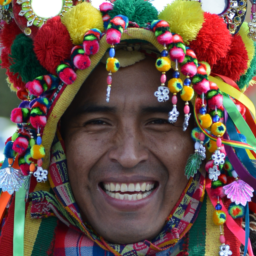
\includegraphics[width=0.245\linewidth]{fig/unsolved/FAST_never_good_01_ref.png} &
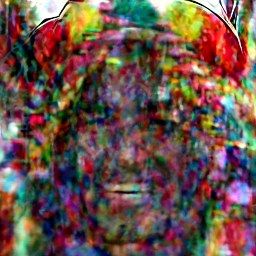
\includegraphics[width=0.245\linewidth]{fig/unsolved/FAST_never_good_01_orc.png} &
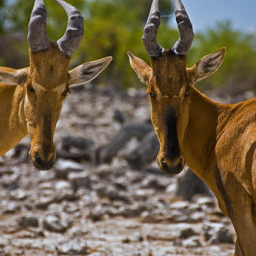
\includegraphics[width=0.245\linewidth]{fig/unsolved/D4_never_orbit_01_ref.png} &
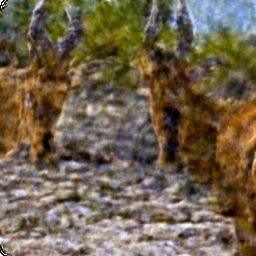
\includegraphics[width=0.245\linewidth]{fig/unsolved/D4_never_orbit_01_orc.png}
\end{tabular}
\caption{\textbf{What no selection can fix.} The best of FAST-DIPS's $64$ runs in any orientation, for an FFHQ image (left) and an ImageNet image (right) without a \good run ($25$ and $20$\,dB). Each is the first of its list in the supplement. On FFHQ, $5$ of the $7$ unsolved images are near misses ($22.8$--$24.7$\,dB)\claim{C-F6}.}
\label{fig:unsolved}
\end{figure}

\paragraph{ImageNet: with four runs, the ground-truth-free pick beats the published oracle.}
DAPS-based samplers give the best reconstructions.
With four runs, $\Eone$ is \good for $72\%$ of the images with DAPS-4K, against $55\%$ with FAST-DIPS and $43\%$ with SITCOM\claim{C-A16}.
Under the published protocol (DAPS-4K, per-metric best of four against the ground truth), DAPS reaches $22.3$\,dB, SSIM $0.52$ and VGG-LPIPS $0.34$ on these images\claim{C-A9}.
This is below the $25.78$\,dB of the DAPS paper~\cite{zhang2025daps} and above an independent rerun ($20.98$\,dB~\cite{kocabas2026pcdaps})\claim{C-P2}, with ground truth and measurements identical to those of the DAPS code\claim{C-A12}.
The per-metric oracle adds $4.2$\,dB to the first run.
The residual pick alone recovers $1.9$\,dB.
With the generic orientation test, it gains $5.1$\,dB and reaches $23.1$\,dB, SSIM $0.53$ and VGG-LPIPS $0.32$, ahead of the oracle on all three metrics without using the ground truth.
With eight runs the two are within $0.01$\,dB\claim{C-A13}.
For FAST-DIPS with $16$ runs, the share of \good outputs is $50\%$ for the residual pick, $65\%$ after the orientation test, $70\%$ for $\Oraw$ and $75\%$ for $\Oorb$\claim{C-R4}.
The test closes $60\%$ of the gap to the orbit oracle; a quarter of the images are not solved in any orientation.

\paragraph{Where the ground-truth-free pick still loses.}
We split the gap between $\Eone$ and $\Oorb$ into two parts (exploratory)\claim{C-E1}.
The selection part counts picks that are \cons or \incons although an orbit-\good run exists.
The orientation part counts picks that are orbit-\good but that the test leaves, or turns, upside down.
On FFHQ, the gap is at most $1.1$ points for every solver, with $8$ to $16$ runs or the four particles of PC-DAPS.
On ImageNet, it is $5.0$ points for DAPS-4K at $K{=}8$, $4.0$ of them orientation, and $2.0$ for PC-DAPS, all orientation.
For FAST-DIPS at $K{=}64$ it is $13.0$ points: $8.0$ from \cons runs that outrank a \good one, and $5.0$ from orientation.
On ImageNet$'$ it is $14.0$ points, half of them orientation, and the generic test adds only $7.9$ points over the residual pick at $K{=}16$, against $17.0$ on ImageNet\claim{C-N4}.
Partial orbit errors, the only ones a channel-wise correction could fix, cost at most $0.6$ points on any panel.
A test closer to the prior helps.
Ordering $\hat x$ and $R_{111}\hat x$ by a paired denoising-loss score, a heuristic proxy for the prior's orientation preference (\cref{sec:setup}; specified before scoring; exploratory), cuts the orientation loss on ImageNet$'$ from $7.0$ to $2.0$ points at $K{=}64$.
At $K{=}16$ it adds $5.3$ points over the generic test ($95\%$ interval $[+1.1,+9.8]$); on ImageNet the two tests are within $1.5$ points\claim{C-X4}.
A learned upright-versus-rotated classifier would be another such proxy and would plug into step~(3) unchanged.

\paragraph{PC-DAPS on the same measurements.}
PC-DAPS~\cite{kocabas2026pcdaps} draws four interacting particles per measurement and reports the mean of their metrics, \ie the quality of a random particle.
On our $180$ FFHQ measurements, that is $28.07$\,dB and a \good image for $79.0\%$ of the images.
Choosing among the same particles by residual and orientation test gives $29.10$\,dB and $84.4\%$, at no extra cost.
The paired $95\%$ intervals of the differences are $[+0.54,+1.61]$\,dB and $[+2.8,+8.5]$ points\claim{C-X1}.
The gain comes from the $18$ images whose four particles are partly \good.
The selection keeps a \good particle in $17$ of them, against $7.25$ expected at random, and ends one image short of the orbit oracle over the four particles\claim{C-X3}.
For scale, one PC-DAPS sample of four particles costs $1{,}920$ nominal denoiser calls and $30.6$\,s on a dedicated GPU; one DAPS-4K run costs $4{,}000$ calls and $66.0$\,s.
DAPS-4K needs two runs, about four times this compute, to reach the same $84.4\%$ with the same selection\claim{C-X2}.
On ImageNet, where many particles are rotated, the same selection raises the share from $30.8\%$ to $53\%$ ($[+14.8,+30.0]$ points) and the PSNR from $17.4$ to $21.5$\,dB.
This is two images short of the orbit oracle; one DAPS-4K run with the same test reaches $55\%$\claim{C-X5}.
